\documentclass[a4paper, 10pt]{article}
\usepackage[utf8x]{inputenc}
\usepackage{graphicx}
\usepackage{geometry}
\usepackage{amsmath}
\usepackage{mathenv}
\usepackage{amssymb}
\usepackage{amsfonts}
\usepackage{mathrsfs}
\usepackage{textcomp}
\geometry{hmargin = 2.5cm, vmargin = 1.5cm}

% OPENING
\title{SY09 - TP03\\Théorie de la décision}
\author{Bertrand Bon - Antoine Hars}

\begin{document}

\maketitle

\section*{Introduction}
Le but de ce tp est de mettre en pratique deux théorie de la décision qui sont le classifieur euclidien et la règle de Bayes.\\

\section*{Exercice 1 : Classifieur euclidien}
Le but de la première partie de ce tp est d'étudier les performances du classifieur euclidien sur des échantillons issus
de deux classes $\omega_{1}$ et $\omega_{2}$ de $\mathbb{R}^{2}$ dont les distributions sont normales et de paramètres
($\mu_{1}$, $\Sigma_{1}$) et ($\mu_{2}$, $\Sigma_{2}$).\\

\subsection*{1. Simulation d'un échantillon.}
En utilisant la fonction \textbf{mvrnorm} de la bibliothèque \textbf{MASS}, nous avons écrit la fonction \textbf{simul} qui nous retourne
un échantillon de taille \textit{n} tiré suivant une proportion $\pi$ d'exemples issus de la classe $\omega_{1}$.
Pour chaque exemple, nous avons, dans un premier temps, tiré au hasard la classe dont il est issu,
avant de le générer en utilisant les paramètres adéquats :\\
\begin{verbatim}
simul <- function (n, pi, mu1, mu2, sigma1, sigma2) {

  result = matrix(nrow = n, ncol = 3)
  for (k in 1:n) {
    rand = sample(0:1, 1)
    result[k, 3] = rand

    if (result[k, 3] == 0) {
      result[k, c(1, 2)] = mvrnorm(1, mu1, sigma1)
    } else {
      result[k, c(1, 2)] = mvrnorm(1, mu2, sigma2)
    }
  }
  return (result)
}
\end{verbatim}
\newpage
\noindent
Nous avons utilisé pour cette fonction les cinq situations suivantes :\\
\textit{n} = 600, $\pi$ = 1/2, $\mu_{1}$ = $(0, 0)^{T}$, $\mu_{2}$ = $(10, 0)^{T}$, $\Sigma_{1}$ = \textit{$a_{1}$}Id et
$\Sigma_{2}$ = \textit{$a_{2}$}Id avec (\textit{$a_{1}$} = 1, \textit{$a_{2}$} = 1),\\(\textit{$a_{1}$} = 1, \textit{$a_{2}$} = 6),
(\textit{$a_{1}$} = 1, \textit{$a_{2}$} = 9), (\textit{$a_{1}$} = 5, \textit{$a_{2}$} = 5) et (\textit{$a_{1}$} = 10, \textit{$a_{2}$} = 10) :\\ \\
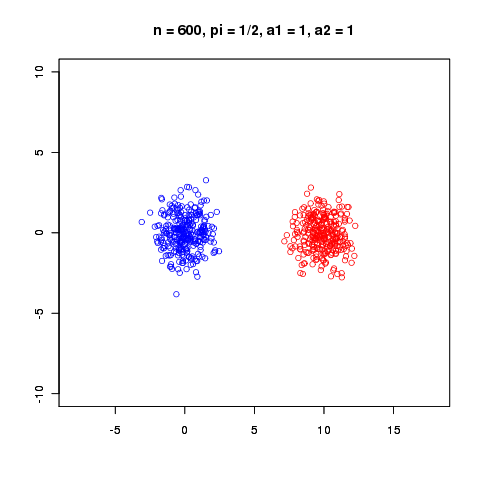
\includegraphics[height = 7cm, width = 7cm]{plots/plot_simul_1.png}
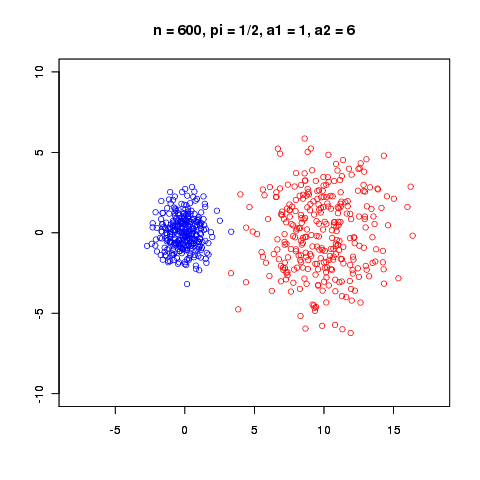
\includegraphics[height = 7cm, width = 7cm]{plots/plot_simul_2.png}\\
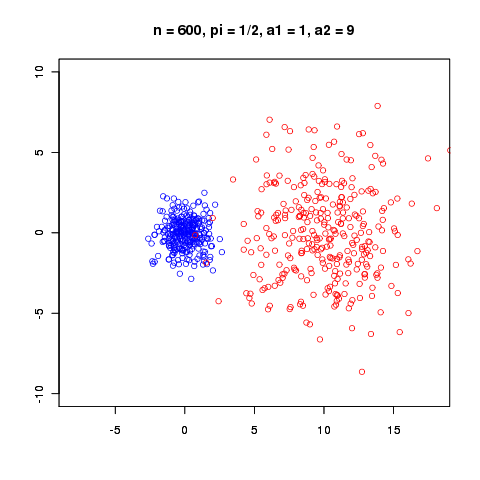
\includegraphics[height = 7cm, width = 7cm]{plots/plot_simul_3.png}
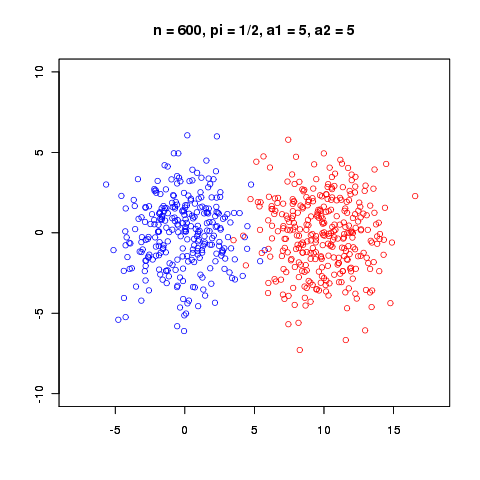
\includegraphics[height = 7cm, width = 7cm]{plots/plot_simul_4.png}\\
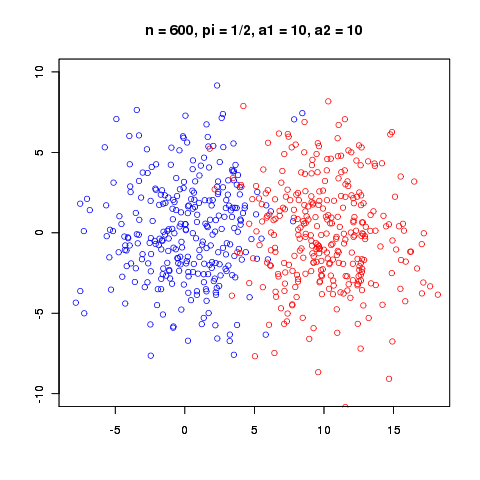
\includegraphics[height = 7cm, width = 7cm]{plots/plot_simul_5.png}
\newpage
\noindent
La première classe est représentée en bleu et la seconde en rouge.\\
Nous pouvons observer que plus la variance $\Sigma$ d'une loi normale augmente, plus l'échantillon lui\\correspondant est dispersé.
Dans ce cas, plus le coefficient \textit{a} de la variance augmente, plus les individus des deux classes ont tendance à se mélanger,
ce qui augmente la probabilité d'erreur entre les deux classes.\\ \\

\subsection*{2. Estimation de la probabilité d'erreur.}
Pour chacun des cinq situations, nous avons cherché à estimer la probabilité d'erreur associée au\\classifieur euclidien.\\
Pour cela, l'échantillon simulé est coupé en deux :
la première moitié forme un échantillon d'apprentissage permettant d'estimer les moyennes $\mu_{1}$ et $\mu_{2}$ et
la seconde moitié forme un ensemble test permettant d'estimer le taux d'erreur.\\ \\
Pour réaliser cela, nous avons écrit plusieurs fonctions :\\ \\
- La fonction \textbf{calculMu} qui va nous calculer les estimations des moyennes $\mu_{1}$ et $\mu_{2}$ de l'échantillon d'apprentissage :\\
\begin{verbatim}
calculMu <- function (ech) {
  
  mu = matrix(c(0, 0, 0, 0), 2, 2)
  tt1 = 0
  tt2 = 0

  for (i in 1:nrow(ech[1:(nrow(ech)), ])) {
    if (ech[i,3] == 0) {
      mu[1] = mu[1] + ech[i,1]
      mu[2] = mu[2] + ech[i,2]
      tt1 = tt1 + 1

    } else {
      mu[3] = mu[3] + ech[i,1]
      mu[4] = mu[4] + ech[i,2]
      tt2 = tt2 + 1
    }
  }

  mu[1] = mu[1] / tt1
  mu[2] = mu[2] / tt1
  mu[3] = mu[3] / tt2
  mu[4] = mu[4] / tt2

  return (mu)
}
\end{verbatim}
$\\ \\$
- La fonction \textbf{regleEuclidienne} retournant la classe retenue par le classifieur euclidien pour une\\observation d'un échantillon :\\
\begin{verbatim}
regleEuclidienne <- function (x, mu1, mu2) {

  if ((abs(mu2["x"] - x[1])) > (abs(mu1["x"] - x[1]))) {
    return (0)
  } else {
    return (1)
  }
}
\end{verbatim}
\newpage
\noindent
- La fonction \textbf{erreurEstimee} qui retourne la probabilité d'erreur estimée sur un échantillon (l'échantillon de test dans notre cas) :\\
\begin{verbatim}
erreurEstimee <- function (ech, regle, mu1, mu2) {

  r = 0
  classement = apply(ech, 1, regle, mu1 = mu1, mu2 = mu2)

  for (i in 1:nrow(ech)) {

    if (classement[i] != ech[i, 3]) {
      r = r + 1
    }
  }

  r = r / nrow(ech) * 100
  return (r)
}
\end{verbatim}
$\\ \\$
Le calcul de la probabilité d'erreur en fonction des estimations de moyennes $\mu_{1}$ et $\mu_{2}$ nous donne les valeurs suivantes :\\ \\
\begin{tabular}{|c|c|c|c|}
\hline
($a_{1}$, $a_{2}$) & $\mu_{1}$ & $\mu_{2}$ & Probabilité d'erreur ($\%$) \\
\hline
(1, 1) & (-0.038, -0.005) & (9.852, -0.146) & 0 \\
\hline
(1, 6) & (0.096, 0.133) & (10.163, -0.361) & 1 \\
\hline
(1, 9) & (-0.127, 0.041) & (9.489, -0.062) & 1.33 \\
\hline
(5, 5) & (-0.145, -0.385) & (10.094, 0.048) & 0 \\
\hline
(10, 10) & (-0.079, 0.160) & (9.798, 0.267) & 3 \\
\hline
\end{tabular}

\newpage
\subsection*{3. Probabilité d'erreur moyenne.}
Nous avons répété les 2 premières questions 10 fois afin d'estimer la moyenne et la variance des résultats obtenus.\\
Pour ce faire, nous avons réaliser une fonction nous permettant d'exécuter toutes les étapes rencontrées précédemment et ce 10 fois de suite 
afin d'obtenir notre probabilité d'erreur moyenne :\\
\begin{verbatim}
erreurMoyenne <- function (n, pi, mu1, mu2, sigma1, sigma2, regle, intervalle) {

  result = matrix(c(0, 0, 0, 0), 1, 4)

  for (i in 1:10) {

    # Création de l'échantillon.
    ech = simul(n, pi, mu1, mu2, sigma1, sigma2)

    # Calcul des estimateurs des moyennes mu1 et mu2
    esti = calculMu(ech[1:(n * pi), ])

    # Calcul de la probabilité d'une erreur.
    e = erreurEstimee(ech[(n * pi + 1):n, ], regle, esti[ ,1], esti[ ,2]) / 100
    result[1] = result[1] + e
    result[2] = e^2 / 10
  }

  # Moyenne
  result[1] = result[1] / 10

  # Variance
  result[2] = result[2] - result[1]^2

  # Écart-type
  e = 10 / (10 - 1) * result[2]

  # Intervalle de Confiance de niveau 5%
  result[3] = result[1] - intervalle * e / sqrt(10)
  result[4] = result[1] + intervalle * e / sqrt(10)

  return (result)
}
\end{verbatim}
$\\\\$
Cette fonction nous permet de récupérer les données suivantes :\\ \\
\begin{tabular}{|c|c|c|c|}
\hline
($a_{1}$, $a_{2}$) & Moyenne empirique & Variance empirique & Intervalle de Confiance \\
\hline
(1, 1) & 0 & 0 & 0 \\
\hline
(1, 6) & 0.009 & -7.067$e^{05}$ & [0.0086, 0.0086] \\
\hline
(1, 9) & 0.025 & -5.139$e^{04}$ & [0.0250, 0.0249] \\
\hline
(5, 5) & 0.013 & -1.733$e^{04}$ & [0.0133, 0.0133] \\
\hline
(10, 10) & 0.065 & -3.737$e^{03}$ & [0.0647, 0.0646] \\
\hline
\end{tabular}$\\\\\\$
Nous pouvons observer, au niveau de l'intervalle de confiance que lorsque nous avons des classes avec une variance élevé,
la moyenne d'erreur augmente du fait que les points sont plus dispersés dans le plan que lorsque la variance des classes est plus faible.

\newpage
\section*{Exercice 2 : Règle de Bayes}
On considère un problème de détection de cibles dans lequel la classe $\mu_{1}$ correspond aux missiles et
la classe $\mu_{2}$ correspond aux avions.
Chaque cible est décrite par deux variables \textit{$X_{1}$} et \textit{$X_{2}$} issues de deux capteurs différents.\\
Chaque variable suit, dans chaque classe, une loi normale avec les paramètres suivants :\\
\textit{$f_{11}$}(\textit{$x_{1}$}) $\sim$ $\mathcal{N}$(-1, 1), \textit{$f_{21}$}(\textit{$x_{1}$}) $\sim$ $\mathcal{N}$(1, 1) et
\textit{$f_{12}$}(\textit{$x_{2}$}) = \textit{$f_{22}$}(\textit{$x_{2}$}) $\sim$ $\mathcal{N}$(0, 1).
On suppose l'indépendance conditionnelle de \textit{$X_{1}$} et \textit{$X_{2}$}.
Les densités conditionnelles du vecteur \textbf{X} = (\textit{$X_{1}$}, \textit{$X_{2}$}$)^T$ sont donc\\
\textit{$f_{1}$}(x) = \textit{$f_{11}$}($x_{1}$)\textit{$f_{12}$}($x_{2}$) dans la classe $\omega_{1}$ et
\textit{$f_{2}$}(x) = \textit{$f_{21}$}($x_{1}$)\textit{$f_{22}$}($x_{2}$) dans la classe $\omega_{2}$.
On suppose que les distributions sont connues et ne sont donc pas estimées à partir d'un échantillon.\\

\subsection*{1. Montrer que les distributions \textit{$f_{1}$} et \textit{$f_{2}$} sont des distributions normales.}
Nous avons donc : \textit{$f_{11}$}(\textit{$x_{1}$}) $\sim$ $\mathcal{N}$(-1, 1), \textit{$f_{21}$}(\textit{$x_{1}$}) $\sim$ $\mathcal{N}$(1, 1) et
\textit{$f_{12}$}(\textit{$x_{2}$}) = \textit{$f_{22}$}(\textit{$x_{2}$}) $\sim$ $\mathcal{N}$(0, 1).\\ \\
Vu que \textit{$X_{1}$} et \textit{$X_{2}$} sont indépendants,
les densités conditionnelles du vecteur \textbf{X} = (\textit{$X_{1}$}, \textit{$X_{2}$}$)^T$ sont donc
\textit{$f_{1}$}(x) = \textit{$f_{11}$}($x_{1}$)\textit{$f_{12}$}($x_{2}$) et
\textit{$f_{2}$}(x) = \textit{$f_{21}$}($x_{1}$)\textit{$f_{22}$}($x_{2}$).\\ \\
La fonction de densité d'une variable aléatoire suivant une loi normale est de la forme \textit{f}(\textit{x}) =
$\frac{1}{\sigma(2\pi)^{\frac{1}{2}}}$\textit{$e^{-\frac{1}{2}(\frac{x - \mu}{\sigma})^{2}}$}\\
Donc \textit{$f_{1}$}(x) = \textit{$f_{11}$}($x_{1}$)\textit{$f_{12}$}($x_{2}$) =
$\frac{1}{\sigma_{11}(2\pi)^{\frac{1}{2}}}$\textit{$e^{-\frac{1}{2}(\frac{x_{1} - \mu_{11}}{\sigma_{11}})^{2}}$} .
$\frac{1}{\sigma_{12}(2\pi)^{\frac{1}{2}}}$\textit{$e^{-\frac{1}{2}(\frac{x_{2} - \mu_{12}}{\sigma_{12}})^{2}}$}$\\\\\\$
\textit{$f_{1}$}(x) = $\frac{1}{2\pi\sigma_{11}\sigma_{12}}$
\textit{$e^{-\frac{1}{2\sigma_{11}^{2}}(x_{1} - \mu_{11})^{2} - \frac{1}{2\sigma_{12}^{2}}(x_{2} - \mu_{12})^{2}}$}$\\\\\\$
\textit{$f_{1}$}(x) = $\frac{1}{2\pi det(\Sigma)^{\frac{1}{2}}}$\textit{$e^-\frac{1}{2}(x - \mu)^{T} \Sigma^{-1}(x - \mu)$}\\
avec $\textit{x} =
\begin{pmatrix}
x_{1} \\
x_{2}
\end{pmatrix}$,
$\mu_{1} = 
\begin{pmatrix}
\mu_{11} \\
\mu_{12}
\end{pmatrix}$,
$\Sigma_{1} = \begin{pmatrix}
\sigma_{11}^{2} & 0 \\
0 & \sigma_{12}^{2}
\end{pmatrix}$ et
$\Sigma_{1}^{-1} =
\begin{pmatrix}
\frac{1}{\sigma_{11}^{2}} & 0 \\
0 & \frac{1}{\sigma_{12}^{2}}
\end{pmatrix}$\\
Nous avons donc \textit{$f_{1}$}(x) $\sim$ $\mathcal{N}$($\mu_{1}$, $\Sigma_{1}$) avec $\mu_{1} =
\begin{pmatrix}
-1 \\
0
\end{pmatrix}$
et $\Sigma_{1} =
\begin{pmatrix}
1 & 0 \\
0 & 1
\end{pmatrix}$\\ \\
Nous appliquons le même raisonnement pour \textit{$f_{2}$} et
nous obtenons un \textit{$f_{2}$}(x) $\sim$ $\mathcal{N}$($\mu_{2}$, $\Sigma_{2}$)\\avec $\mu_{2} =
\begin{pmatrix}
1 \\
0
\end{pmatrix}$
et $\Sigma_{2} =
\begin{pmatrix}
1 & 0 \\
0 & 1
\end{pmatrix}$
\newpage

\subsection*{2. Générer un échantillon de \textit{n} réalisations issues des deux classes $\omega_{1}$ et $\omega_{2}$.}
Pour générer un échantillon de \textit{n}n réalisations issues des deux classes $\omega_{1}$ et $\omega_{2}$ en proportions égales\\
($\pi_{1}$ = $\pi_{2}$ = 0.5), nous avons utilisé la fonction \textbf{simul} écrite précédemment.\\
Pour chacun des échantillons, nous avons ensuite déterminé les estimations des différents paramètres de \textit{$f_{1}$} et \textit{$f_{2}$}.\\
Pour les valeurs de \textit{n} suivantes : 10, 100, 1000, 10 000, 100 000, nous obtenons donc les graphiques suivants :\\
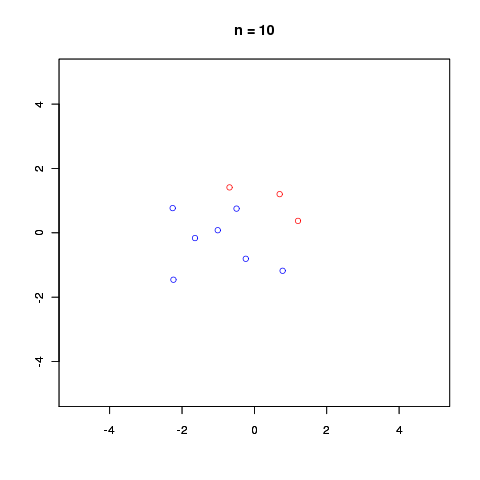
\includegraphics[height = 7cm, width = 7cm]{plots/plot_simul_6.png}
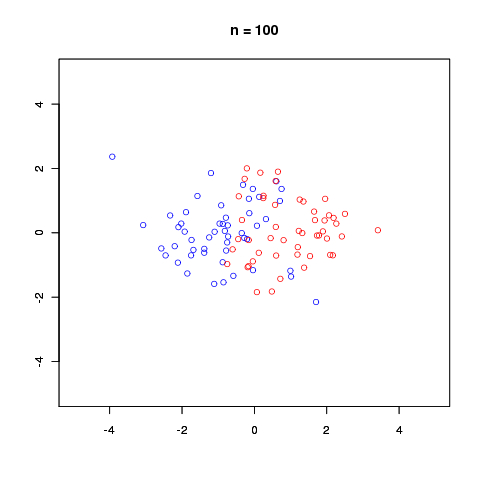
\includegraphics[height = 7cm, width = 7cm]{plots/plot_simul_7.png}\\
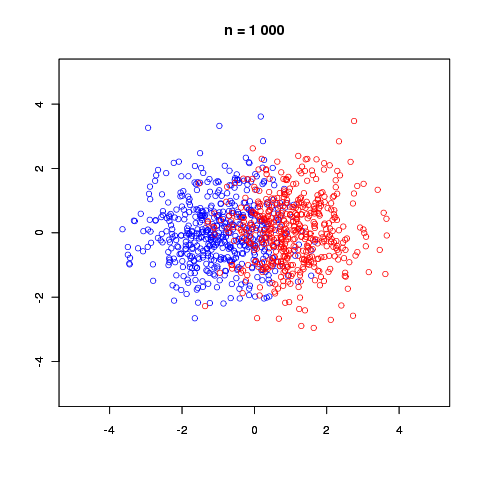
\includegraphics[height = 7cm, width = 7cm]{plots/plot_simul_8.png}
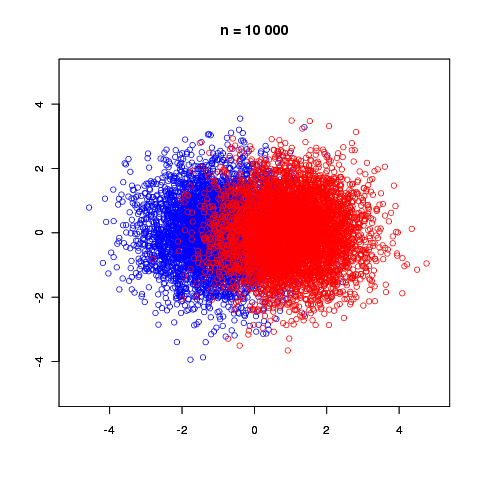
\includegraphics[height = 7cm, width = 7cm]{plots/plot_simul_9.png}\\
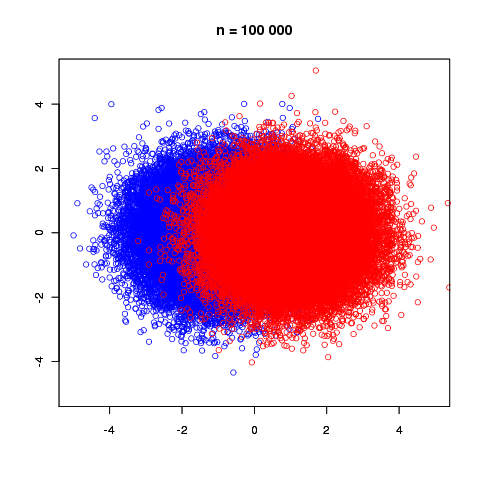
\includegraphics[height = 7cm, width = 7cm]{plots/plot_simul_10.png}
\newpage
\noindent
Nous pouvons observer les estimations des différents paramètres de \textit{$f_{1}$} et de \textit{$f_{2}$} dans le tableau suivant :\\ \\
\begin{tabular}{|c|c|c|c|c|}
\hline
Échantillon & $\bar{\mu_{1}}$ & $\bar{\Sigma_{1}}$ & $\bar{\mu_{2}}$ & $\bar{\Sigma_{2}}$ \\
\hline
10 & $\begin{pmatrix} -0.570 \\ -0.584 \end{pmatrix}$ & $\begin{pmatrix} 0.762 & 0.302 \\ 0.302 & 0.354 \end{pmatrix}$ &
$\begin{pmatrix} 1.883 \\ 0.327 \end{pmatrix}$ & $\begin{pmatrix} 1.954 & -0.092 \\ -0.091 & 0.700 \end{pmatrix}$ \\
\hline
100 & $\begin{pmatrix} -1.164 \\ 0.114 \end{pmatrix}$ & $\begin{pmatrix} 0.802 & 0.156 \\ 0.156 & 1.121 \end{pmatrix}$ &
$\begin{pmatrix} 0.575 \\ 0.094 \end{pmatrix}$ & $\begin{pmatrix} 1.359 & 0.200 \\ 0.200 & 0.937 \end{pmatrix}$ \\
\hline
1 000 & $\begin{pmatrix} -1.0854 \\0.006 \end{pmatrix}$ & $\begin{pmatrix} 1.011 & -0.053 \\ -0.053 & 0.830 \end{pmatrix}$ &
$\begin{pmatrix} 0.961 \\ 0.051 \end{pmatrix}$ & $\begin{pmatrix} 1.099 & 0.113 \\ 0.113 & 0.946 \end{pmatrix}$ \\
\hline
10 000 & $\begin{pmatrix} -1.003 \\ -0.009 \end{pmatrix}$ & $\begin{pmatrix} 0.993 & 0.027 \\ 0.027 & 0.982 \end{pmatrix}$ &
$\begin{pmatrix} 0.987 \\ 0.012 \end{pmatrix}$ & $\begin{pmatrix} 0.974 & 0.010 \\ 0.010 & 0.967 \end{pmatrix}$ \\
\hline
100 000 & $\begin{pmatrix} -1.002 \\ 0.001 \end{pmatrix}$ & $\begin{pmatrix} 0.995 & 0.000 \\ 0.000 & 0.997 \end{pmatrix}$ &
$\begin{pmatrix} 1.001 \\ 0.003 \end{pmatrix}$ & $\begin{pmatrix} 1.011 & 0.000 \\ 0.000 & 1.00 \end{pmatrix}$ \\
\hline
\end{tabular}\\ \\
Nous avons pu observer que plus n était grand, plus on se rapprochait de la valeur théorique.\\ \\
% TODO Récupérer Sigma1 et Sigma2

\subsection*{3. Montrer que les courbes d'iso-densité sont des cercles.}
Calculer les courbes d'iso-densité revient à résoudre l'équation suivante :\\
\textit{$f_{w_{1}}$(x) = K} où \textit{K} est une constante.\\ \\
Dans le cas de \textit{$f_{1}$(x)} = $K_{1}$\\
$\frac{1}{2}(x - \mu)^{T} (x -\mu) = -ln(2\pi K)$\\
$\Leftrightarrow (x_{1} - \mu_{1})^{2} + (x_{2} - \mu_{2})^{2} = -2ln(2\pi K_{1})$\\
$\Leftrightarrow (x{1} + 1)^{2} + x_{2}^{2} = -2ln(2\pi K_{1})$\\
Nous avons donc finalement un cercle de centre $\mu_{1}$ = $\begin{pmatrix} -1 \\ 0 \end{pmatrix}$ et de rayon $\sqrt{-2ln(2\pi K_{1}}$.\\
Dans le cas de \textit{$f_{2}$(x)} = $K_{2}$,
nous obtenons un cercle de centre $\mu_{1}$ = $\begin{pmatrix} 1 \\ 0 \end{pmatrix}$ et de rayon $\sqrt{-2ln(2\pi K_{2}}$.\\ \\ \\
Nous avons donc obtenu un graphique de la forme suivante :\\
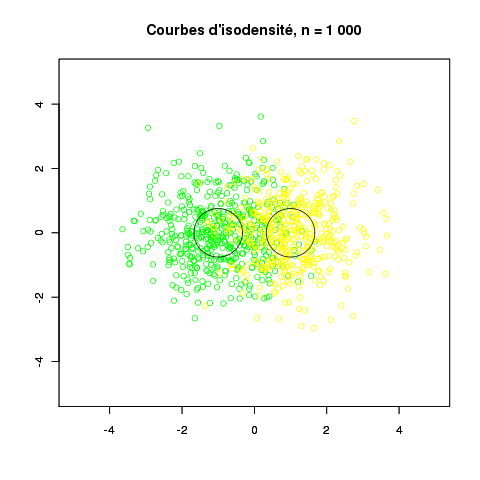
\includegraphics[height = 7cm, width = 7cm]{plots/plot_isodensite.png}\\
Pour ce graphique, nous avons choisi de prendre \textit{$K_{1}$} = \textit{$K_{2}$} = 0.2.
Nous pouvons aussi confirmer\\visuellement ce que la partie calcul à montrer,
à savoir que ces courbes d'iso-densité sont des cercles de\\rayon = 0.671 dans notre cas.
\newpage

\subsection*{4. Règle de Bayes.}
Soient $\pi_{1}$ et $\pi_{2}$ les probabilité à priori des deux classes,
et \textit{$c_{lk}$} le coût associé au choix de l'action \textit{$a_{l}$} lorsque la vraie classe est $\omega_{k}$.
On suppose \textit{$c_{11}$} = \textit{$c_{22}$} = 0.

\subsubsection*{(a) Donner l'expression de la règle de Bayes $\delta^{*}$ pour ce problème.}
La règle de Bayes s'écrit de la manière suivante :\\
$\delta^{*}(x) =
\begin{cases} 
  a_{1} & si \frac{f_{1}(x)}{f_{2}(x)} > \frac{c_{12}\pi_{2}}{c_{21}\pi{1}} \\
  a_{2} & sinon.
\end{cases}$\\ \\
Les coûts sont définis ainsi :\\ \\
\begin{tabular}{|c|c|c|}
\hline
& $\omega_{1}$ & $\omega_{2}$ \\
\hline
$a_{1}$ & $c_{11}$ & $c_{12}$ \\
\hline
$a_{2}$ & $c_{21}$ & $c_{22}$ \\
\hline
\end{tabular}\\ \\

\subsubsection*{(b) Tracer les frontières de décision correspondantes dans le plan (\textit{$X_{1}$}, \textit{$X_{2}$}).}
- Dans le cas où \textit{$c_{12}$} = \textit{$c_{21}$} = 1, $\pi_{1}$ = $\pi_{2}$ :\\
Nous pouvons écrire la règle de Bayes pour ce cas donc nous avons $\delta^{*}$ = \textit{$a_{1}$}
$\Leftrightarrow$ \textit{$f_{1}$(x)} $>$ \textit{$f_{2}$(x)}.\\
Ici, nous trouvons que \textit{$f_{1}$(x)} = \textit{$f_{2}$(x)}
$\Leftrightarrow$ (\textit{x} + 1$)^{2}$ = (\textit{x} - 1$)^{2}$
$\Leftrightarrow$ \textit{x} = 0\\
La frontière de décision est la droite d'équation \textit{x} = 0 dans ce cas de figure.\\ \\
- Dans le cas où \textit{$c_{12}$} = 10, \textit{$c_{21}$} = 1, $\pi_{1}$ = $\pi_{2}$ :\\
Nous pouvons écrire la règle de Bayes pour ce cas donc nous avons $\delta^{*}$ = \textit{$a_{1}$}
$\Leftrightarrow$ \textit{$f_{1}$(x)} $>$ u.\textit{$f_{2}$(x)}.\\
$\frac{f_{1}(x)}{f_{2}(x)} <$ 10\\
$\Leftrightarrow e^{-2(x)} <$ 10\\
$\Leftrightarrow x = -\frac{ln(10)}{2}$\\ \\
La frontière de décision, pour ce cas, la droite d'équation $x = -\frac{ln(10)}{2}$, soit approximativement la droite d'équation $x = -1.15$\\ \\
- Dans le cas où \textit{$c_{12}$} = \textit{$c_{21}$} = 1, $\pi_{2}$ = 10$\pi_{1}$ :\\
Nous pouvons écrire la règle de Bayes pour ce cas donc nous avons $\delta^{*}$ = \textit{$a_{1}$}
$\Leftrightarrow$ \textit{$f_{1}$(x)} $>$ u.\textit{$f_{2}$(x)}.\\
$\frac{f_{1}(x)}{f_{2}(x)} <$ 10\\
$\Leftrightarrow e^{-2(x)} <$ 10\\
$\Leftrightarrow x = -\frac{ln(10)}{2}$\\ \\
La frontière de décision, pour ce cas, la droite d'équation $x = -\frac{ln(10)}{2}$, soit approximativement la droite d'équation $x = -1.15$
comme pour le cas précédent.
\newpage
\noindent
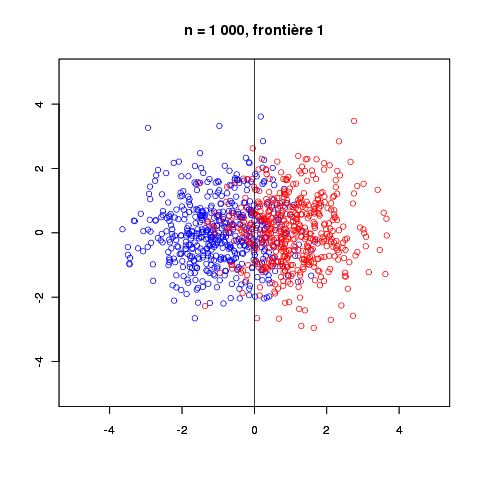
\includegraphics[height = 7cm, width = 7cm]{plots/plot_frontiere_1.png}
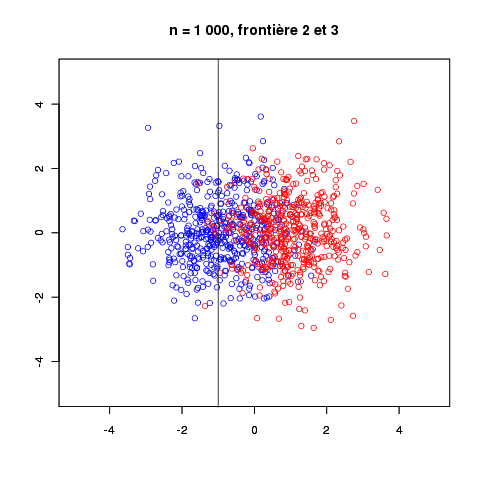
\includegraphics[height = 7cm, width = 7cm]{plots/plot_frontiere_2.png}\\
À travers ces deux graphiques, nous pouvons dire que dans le premier cas, les erreurs de la première et de la deuxième classe sont du même ordre.
Aucune des deux n'est plus pénalisée par rapport à cet frontière.\\ \\
Pour le second et troisième cas, le coût d'erreur de la première classe, est plus grand grand que celui de la seconde classe.
Par conséquent, la règle a tendance à minimiser les erreurs de la seconde classe.\\ \\

\subsubsection*{(c) Donner une estimation des risques $\alpha$ et $\beta$.}
Pour évaluer une estimation des risques $\alpha$ = $\mathbb{P}$($\delta^{*}$(\textbf{X}) = \textit{$a_{2}$}$\mid\omega_{1}$) et
$\beta$ = $\mathbb{P}$($\delta^{*}$(\textbf{X}) = \textit{$a_{1}$}$\mid\omega_{2}$), nous utilisons la fonction \textbf{simul} écrite
en début de tp.\\
Ces risques sont définis par $\alpha$ = $\mathcal{P}$($\delta^{*}$(\textit{x}) = $a_{2}\mid\omega_{1}$) et
$\beta$ = $\mathcal{P}$($\delta^{*}$(\textit{x}) = $a_{1}\mid\omega_{2}$).\\ \\
Nous obtenons ainsi les données suivantes :\\ \\
\begin{tabular}{|c|c|c|}
\hline
& $\alpha$ & $\beta$ \\
\hline
$c_{12} = c_{21} = 1, \pi_{1} = \pi_{2}$ & 0.16 & 0.17 \\
\hline
$c_{12} = 10, c_{21} = 1, \pi_{1} = \pi_{2}$ & 0.53 & 0.01 \\
\hline
$c_{12} = c_{21} = 1, \pi_{2} = 10 \pi_{1}$ & 0.70 & 0.03 \\
\hline
\end{tabular}\\ \\


Dans le premier cas, nous pouvons observer que les estimateurs des risques $\alpha$ et $\beta$ sont très proches.\\
Dans le deuxième et le troisième cas, $\beta$ est plus petit que $\alpha$.


\section*{Conclusion}
Durant ce TP, nous avons eu la possibilité d'utiliser deux méthodes de classification supervisée :\\
le classifieur euclidien, l'un des plus simples pour se baser un ensemble d'apprentissage pour déterminer\\le centre de classes.
Cette simplicité vient de paire avec une limitation du coté de la gestion des\\distributions très distribuées dans le plan.\\
puis la règle de Bayes qui permet de contrôler les risques ce qui ajoute une gestion des erreurs plus poussée.
Avec cette méthode, nous avons pu voir que nous pouvions réduire le risque d'erreur au lieu du nombre d'erreurs,
nous permettant ainsi de priviliéger ou non un certain type d'erreur par rapport à d'autres.

\end{document}
